\chapter{Resultados e Discussão}
\label{chap4}
\section{Geração dos Dados}
\subsection{Simulação}
A figura \ref{fig:sim_inputs_raw} ilustra os sinais de entrada ($f$ e $I_r$) de treino e teste da simulação, utilizando os valores descritos na tabela \ref{tab:params_aprbs}:

\begin{figure}[hbt!]
    \centering
    \includegraphics[width=0.8\linewidth]{Imagens/chap04/sim_inputs_train_raw.png}
    \hfill
    \includegraphics[width=0.8\linewidth]{Imagens/chap04/sim_inputs_test_raw.png}
    \caption{Sinais de entrada de treino (acima) e teste (abaixo) da simulação do sistema. O sinal foi truncado em 100 amostras para facilitar a visualização. Fonte: Autor}
    \label{fig:sim_inputs_raw}
\end{figure}

A figura \ref{fig:sim_outputs_raw} ilustra os sinais de saída ($w_e$ e $h$) de treino e teste da simulação

\begin{figure}[hbt!]
    \centering
    \includegraphics[width=0.8\linewidth]{Imagens/chap04/sim_outputs_train_raw.png}
    \hfill
    \includegraphics[width=0.8\linewidth]{Imagens/chap04/sim_outputs_test_raw.png}
    \caption{Saídas de saída de treino (acima) e teste (abaixo) da simulação. O sinal foi truncado em 100 amostras para facilitar a visualização. Fonte: Autor}
    \label{fig:sim_outputs_raw}
\end{figure}

\subsection{Dados experimentais}
A figura \ref{fig:exp_inputs_raw} ilustra a entrada $f$ de treino e teste dos dados experimentais:
\begin{figure}[hbt!]
    \centering
    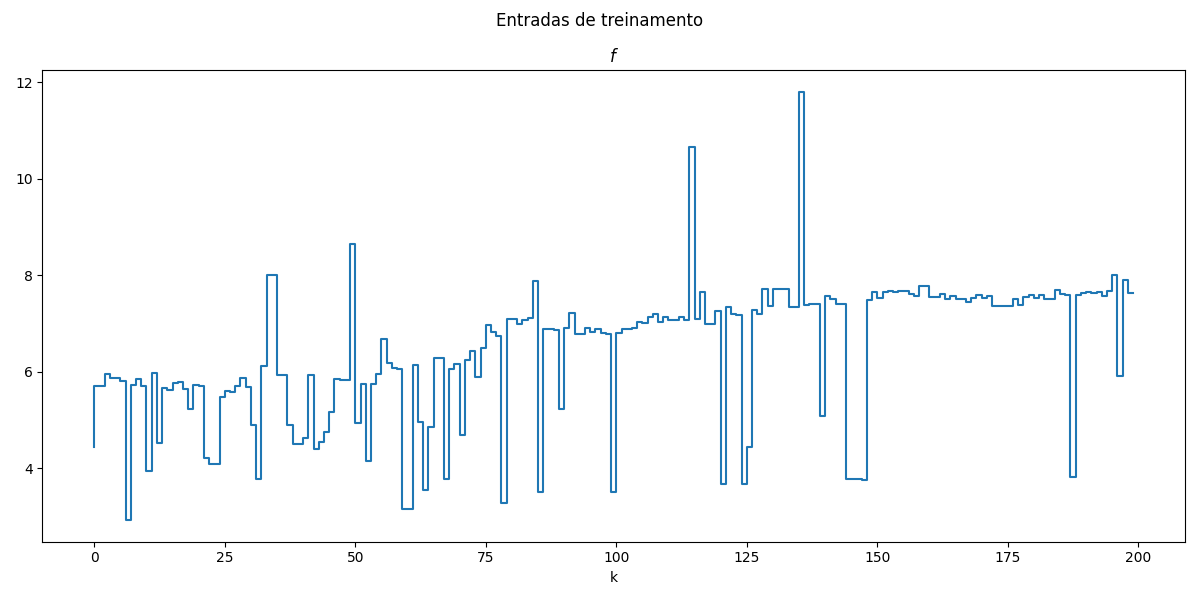
\includegraphics[width=0.8\linewidth]{Imagens/chap04/experiment_inputs_train_raw.png}
    \hfill
    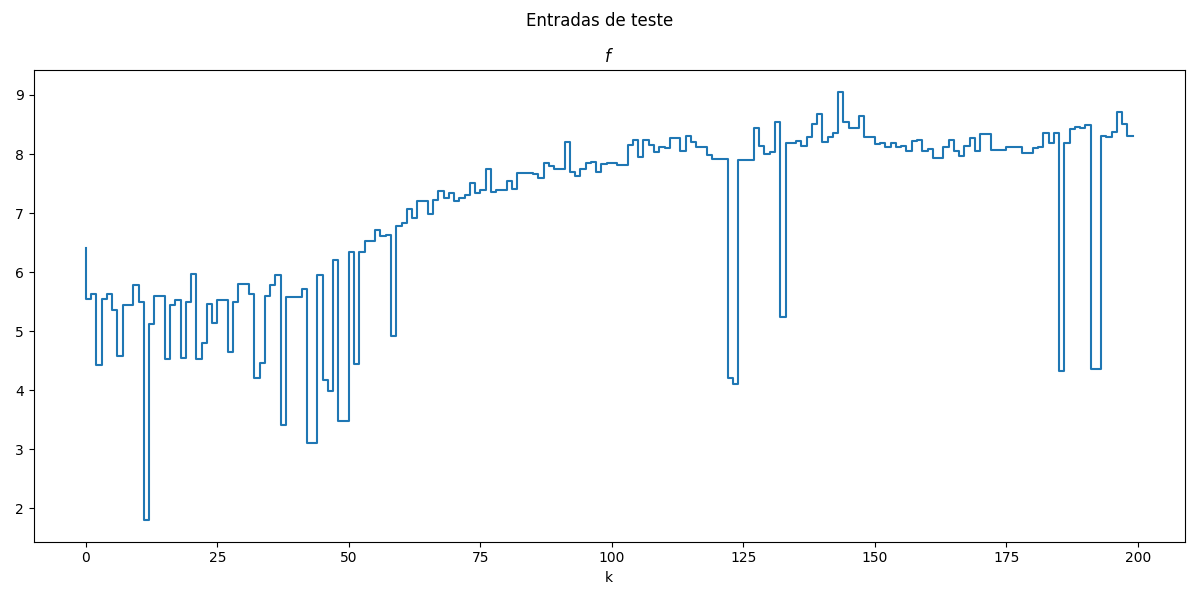
\includegraphics[width=0.8\linewidth]{Imagens/chap04/experiment_inputs_test_raw.png}
    \caption{Entrada de treino (acima) e teste (abaixo) dos dados experimentais. Fonte: Autor}
    \label{fig:exp_inputs_raw}
\end{figure}

A figura \ref{fig:exp_outputs_raw} ilustra a saída $w_e$ de treino e teste dos dados experimentais:
\begin{figure}[hbt!]
    \centering
    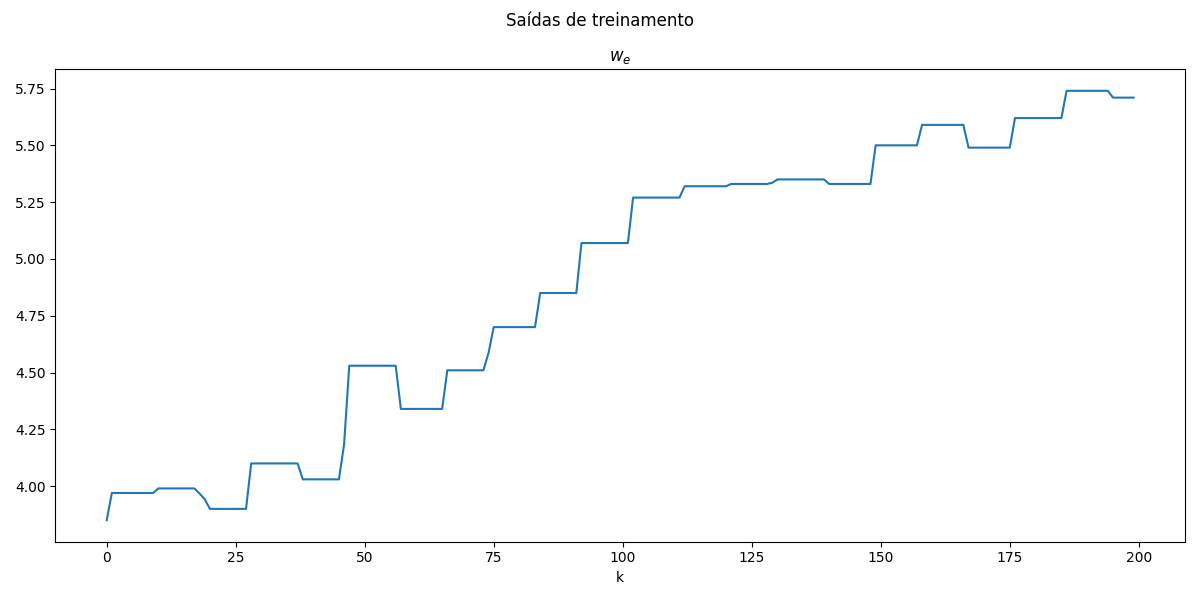
\includegraphics[width=0.8\linewidth]{Imagens/chap04/experiment_outputs_train_raw.png}
    \hfill
    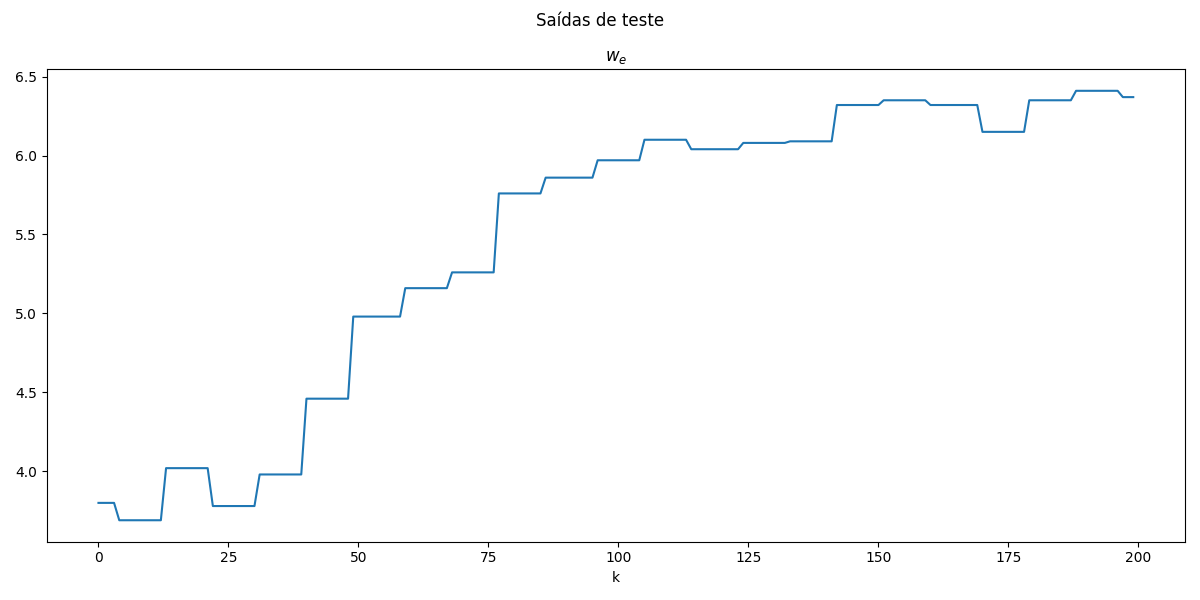
\includegraphics[width=0.8\linewidth]{Imagens/chap04/experiment_outputs_test_raw.png}
    \caption{Saída de treino (acima) e teste (abaixo) dos dados experimentais. Fonte: Autor}
    \label{fig:exp_outputs_raw}
\end{figure}

\newpage
\section{Tratamento dos Dados}
\subsection{Simulação}
As figuras \ref{fig:sim_inputs} e \ref{fig:sim_outputs} ilustram a normalização min-max e média-desvio padrão, respectivamente, das entradas e saídas do processo.

\begin{figure}[hbt!]
    \centering
    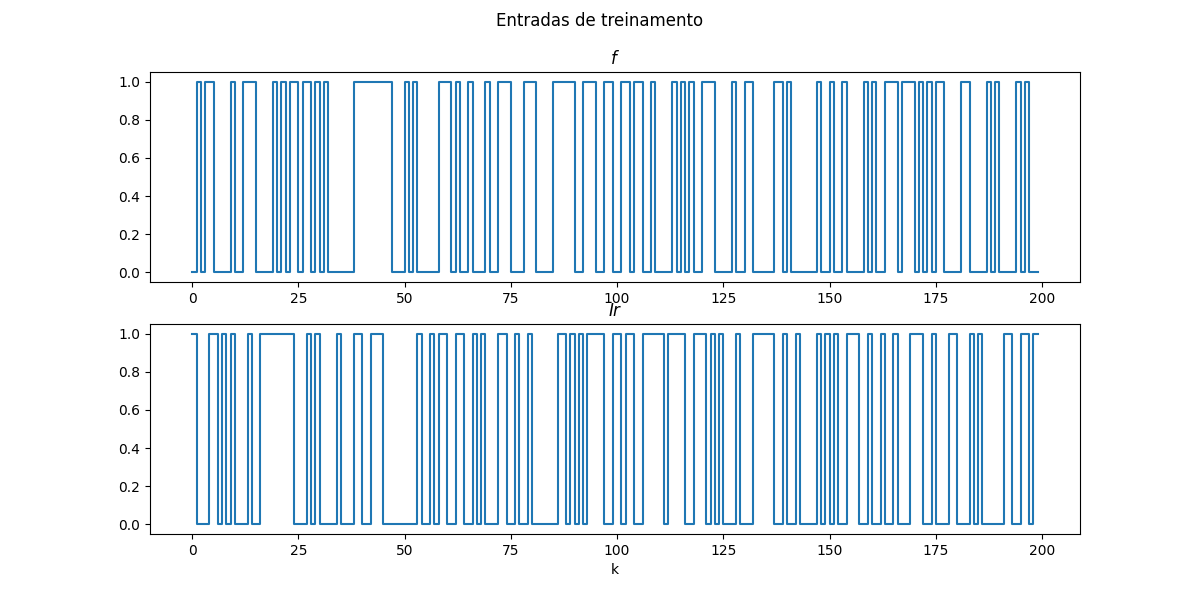
\includegraphics[width=0.8\linewidth]{Imagens/chap04/simulation_inputs_train.png}
    \hfill
    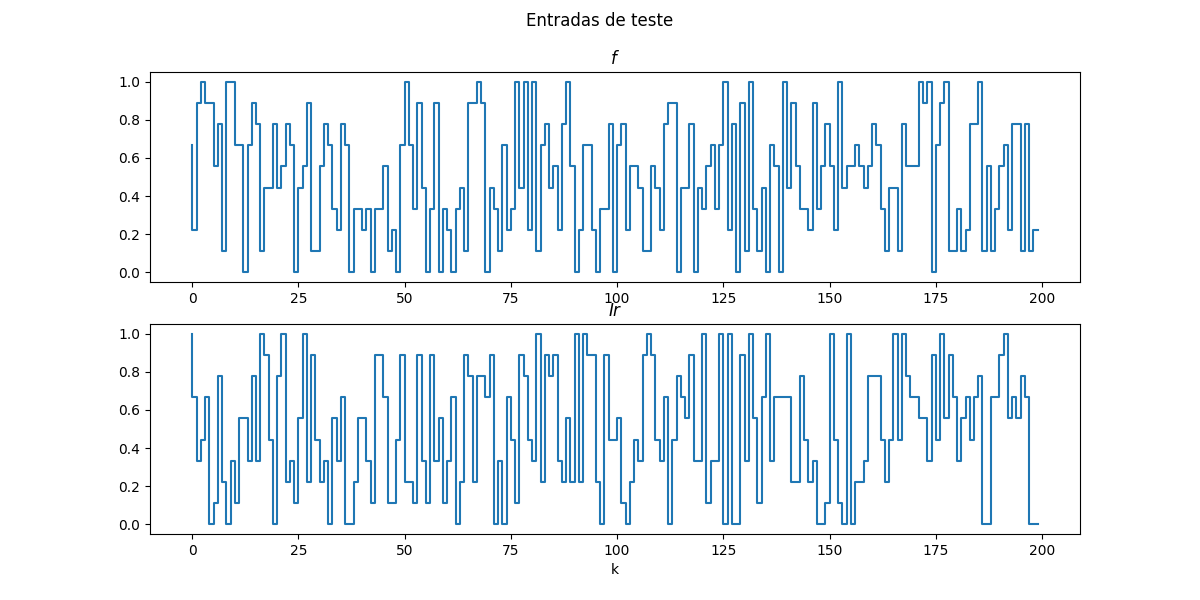
\includegraphics[width=0.8\linewidth]{Imagens/chap04/simulation_inputs_test.png}
    \caption{Sinais normalizados de treino (cima) e teste (baixo) utilizados como entrada da simulação do sistema.
 O sinal foi truncado em 100 amostras para facilitar a visualização. Fonte: Autor}
    \label{fig:sim_inputs}
\end{figure}

\begin{figure}[hbt!]
    \centering
    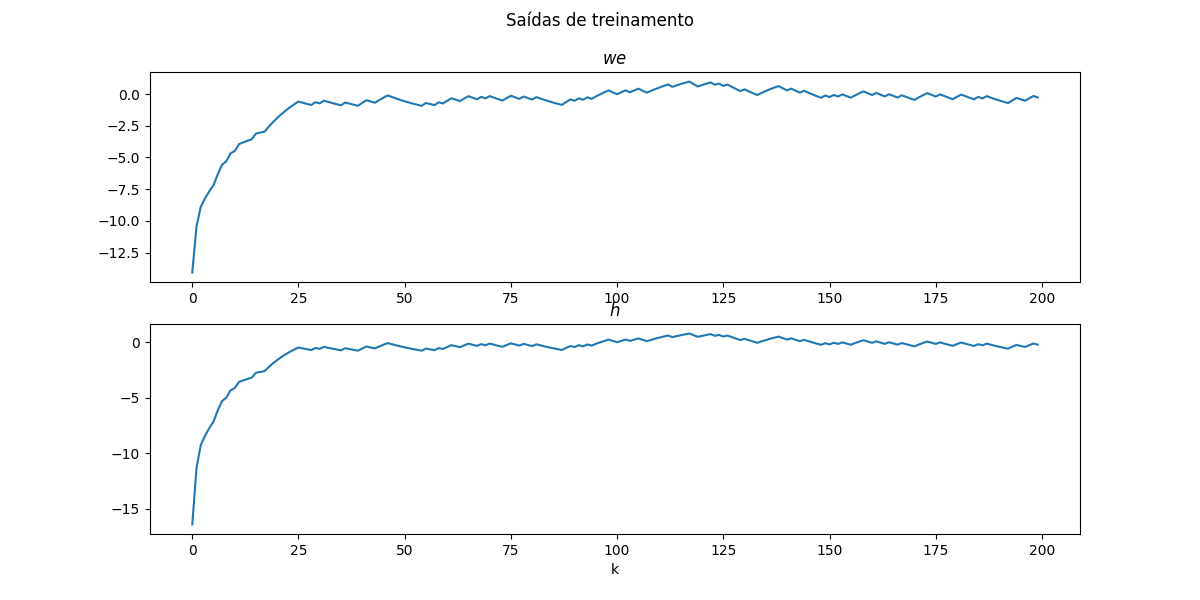
\includegraphics[width=0.8\linewidth]{Imagens/chap04/simulation_outputs_train.png}
    \hfill
    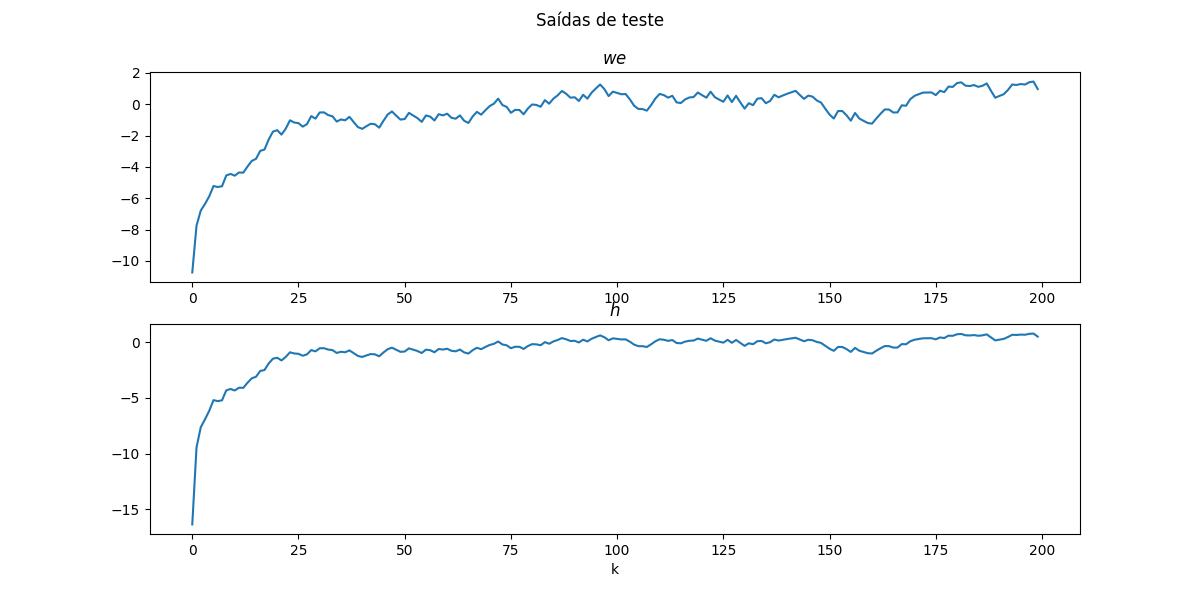
\includegraphics[width=0.8\linewidth]{Imagens/chap04/simulation_outputs_test.png}
    \caption{Saídas normalizadas de treino (cima) e teste (baixo) da simulação. O sinal foi truncado em 100 amostras para facilitar a visualização. Fonte: Autor}
    \label{fig:sim_outputs}
\end{figure}

\subsection{Dados experimentais}
As figuras \ref{fig:exp_inputs} e \ref{fig:exp_outputs} ilustram a normalização min-max e média-desvio padrão, respectivamente, das entradas e saídas dos dados experientais.

\begin{figure}[hbt!]
    \centering
    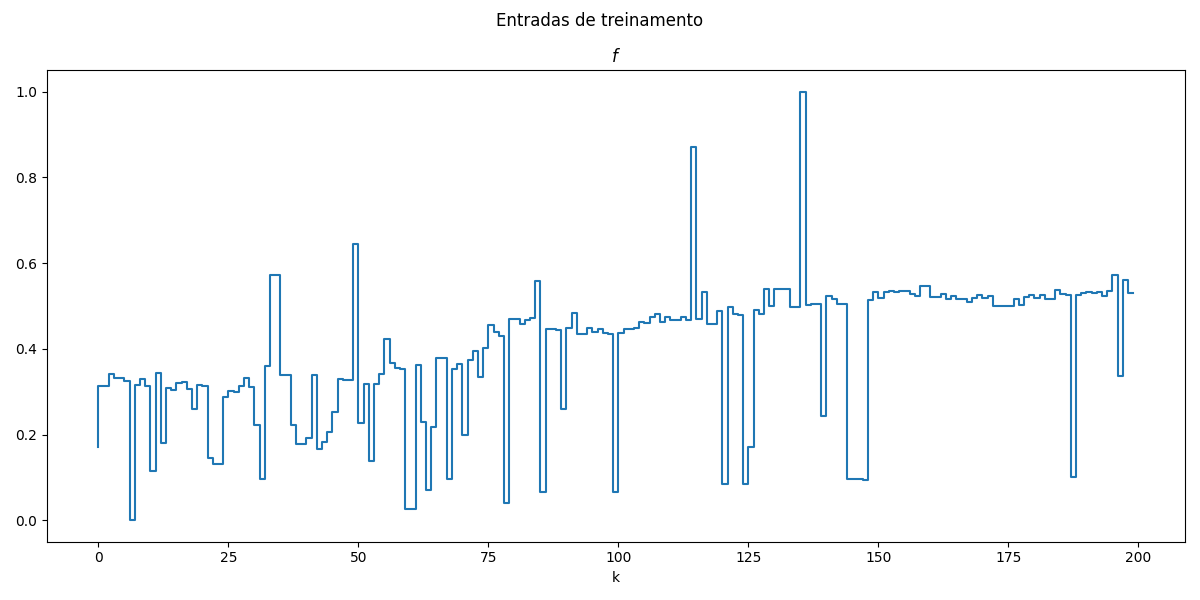
\includegraphics[width=0.8\linewidth]{Imagens/chap04/experiment_inputs_train.png}
    \hfill
    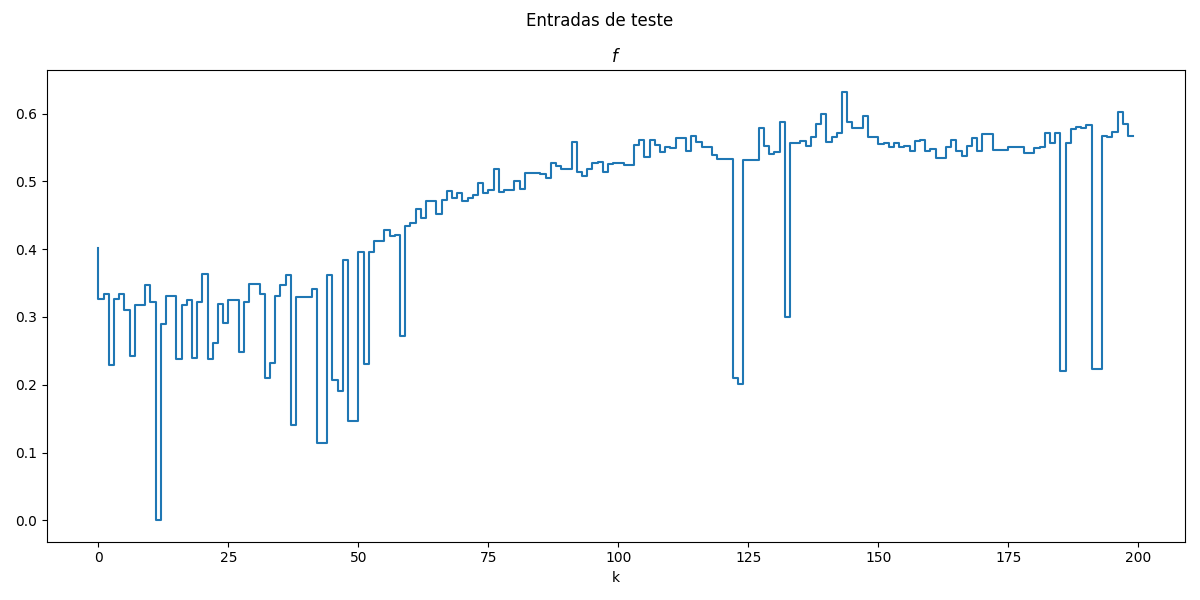
\includegraphics[width=0.8\linewidth]{Imagens/chap04/experiment_inputs_test.png}
    \caption{Sinais normalizados de treino (cima) e teste (baixo) de entrada dos dados experimentais.
 O sinal foi truncado em 100 amostras para facilitar a visualização. Fonte: Autor}
    \label{fig:exp_inputs}
\end{figure}

\begin{figure}[hbt!]
    \centering
    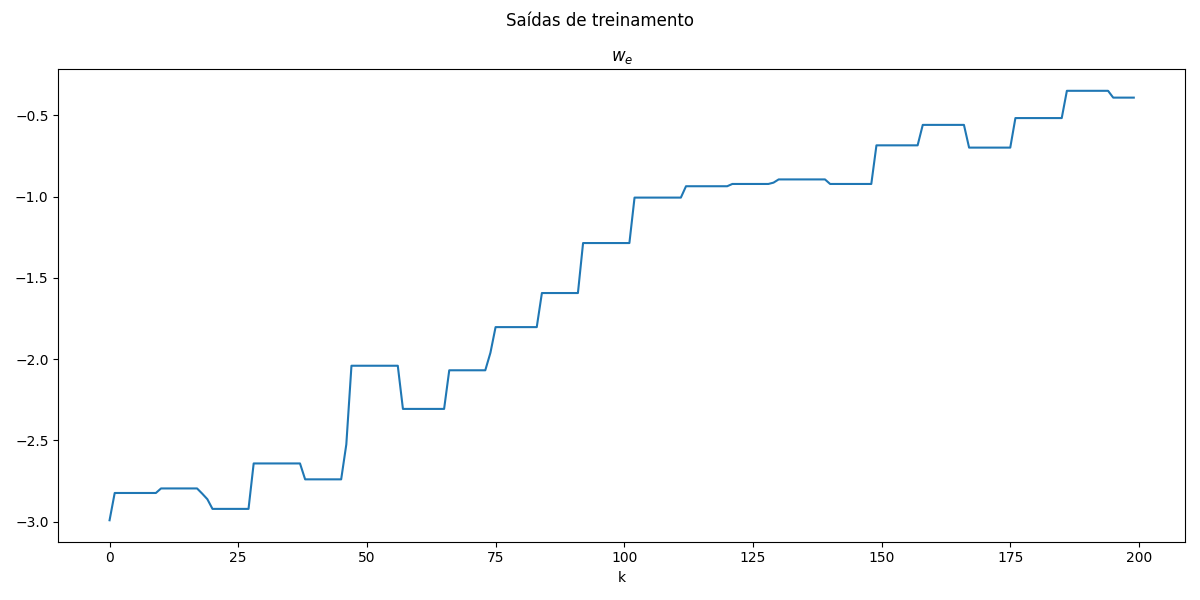
\includegraphics[width=0.8\linewidth]{Imagens/chap04/experiment_outputs_train.png}
    \hfill
    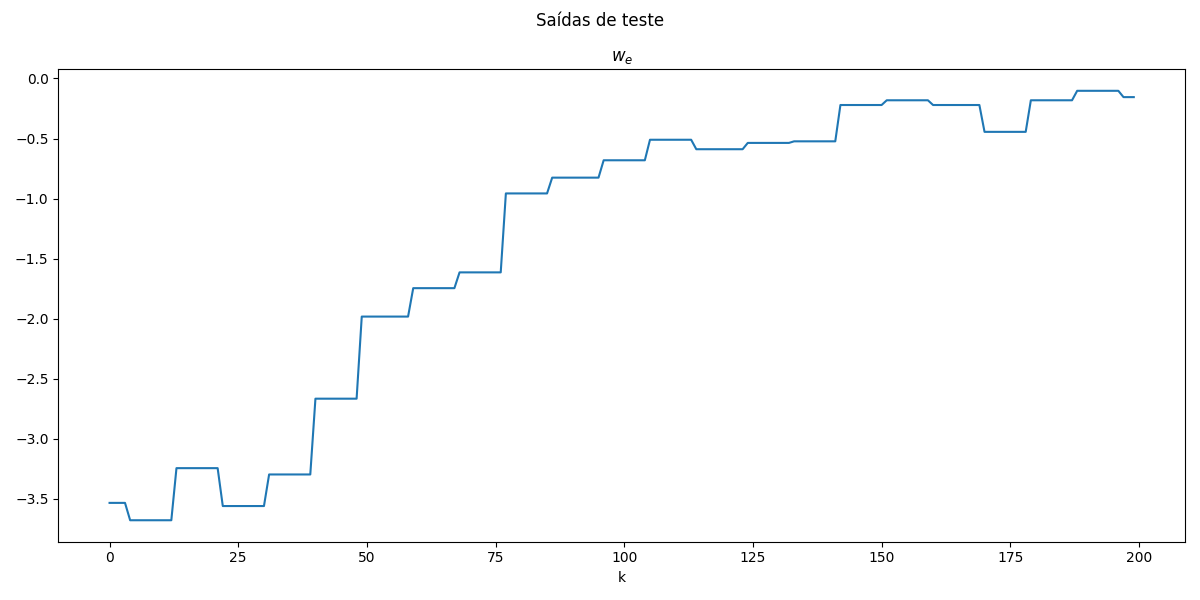
\includegraphics[width=0.8\linewidth]{Imagens/chap04/experiment_outputs_test.png}
    \caption{Sinais normalizados de treino (cima) e teste (baixo) de saída dos dados experimentais.
    \label{fig:exp_outputs}
\end{figure}

\section{Modelagem da rede LSTM}
\subsection{Ajuste dos hiperparâmetros}
\subsubsection{Simulação}
As figuras \ref{fig:sim_hp_metrics} ilustram os resultados do treinamento dos hiperparâmetros $P$, $Q$ e tamanho de batelada.

\begin{figure}[hbt!]
    \centering
    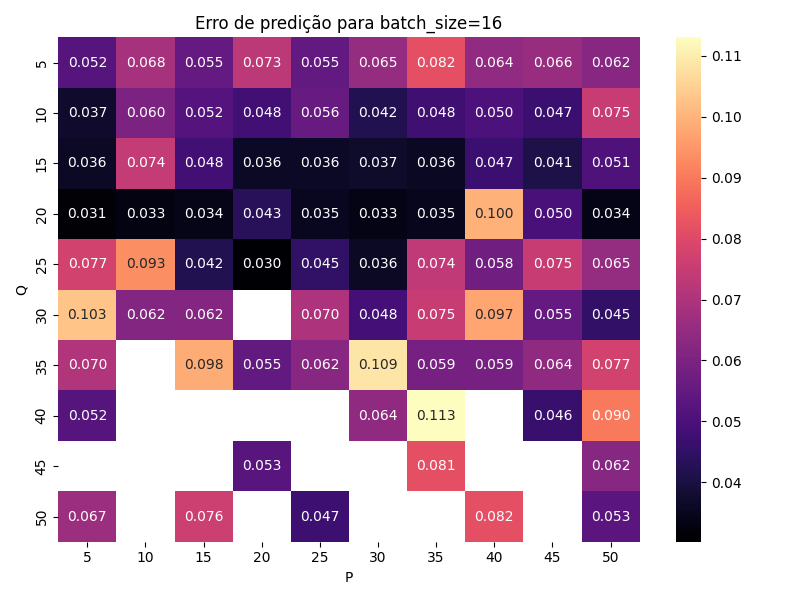
\includegraphics[width=0.7\linewidth]{Imagens/chap04/simulation_hp_metrics_16.png}
    \hfill
    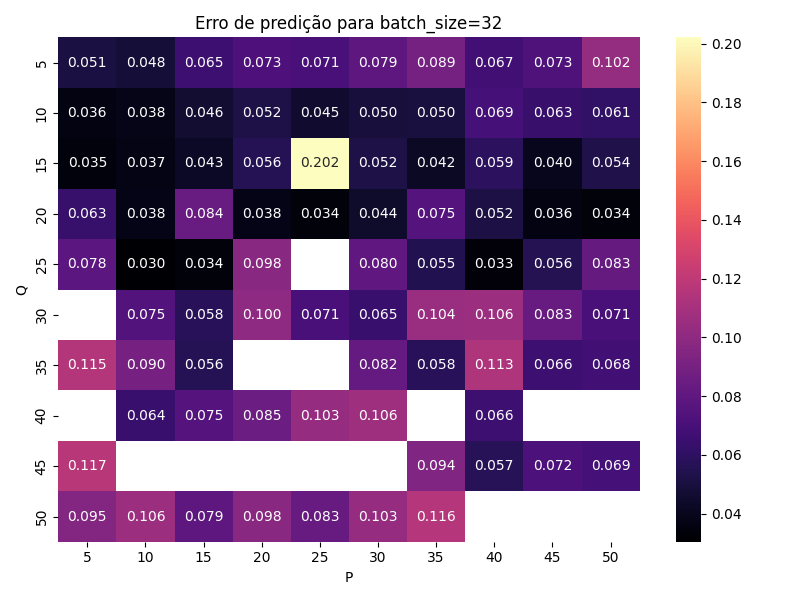
\includegraphics[width=0.7\linewidth]{Imagens/chap04/simulation_hp_metrics_32.png}
    \hfill
    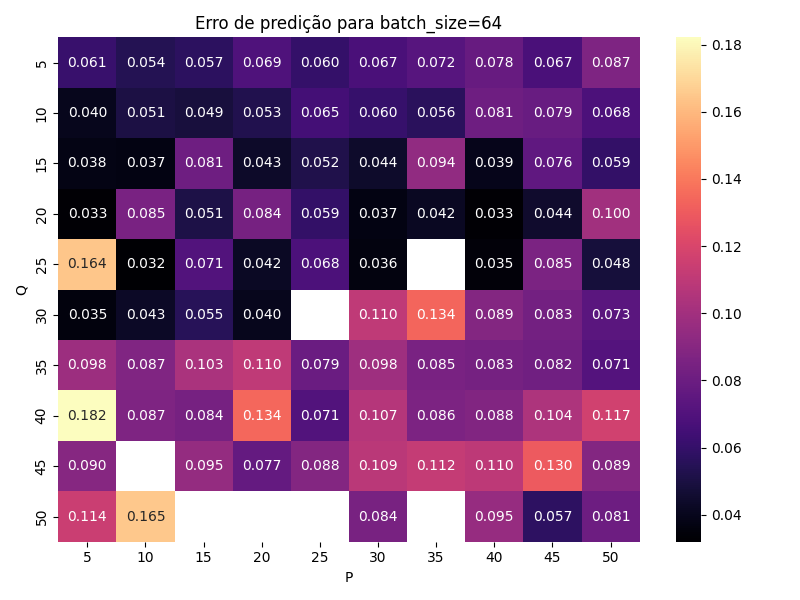
\includegraphics[width=0.7\linewidth]{Imagens/chap04/simulation_hp_metrics_64.png}
    \caption{Mapa de calor indicando o erro RMS para diferentes valores de $P$ e $Q$ e para tamanho de batelada 16 (esquerda), 32 (direita) e 64 (baixo). Fonte: Autor}
    \label{fig:sim_hp_metrics}
\end{figure}

O melhor resultado é o de $(P,Q,batch\_size)=(20,25,16)$, cujo RMSE é de 0.03.  Porém, a rede com hiperparâmetros $(P,Q,batch\_size)=(5,20,16)$ performou quase tão bem, como RMSE de 0.031, e utiliza uma janela significante menor de pontos históricos de entrada (5) e saída (20). Isso significa que o número de parâmetros dessa rede é inferior, o que acelera seu treinamento, portanto foi a rede escolhida. Os valores vazios são de treinamentos que retornaram um erro que é um outlier e foram removidos para auxiliar na visualização do mapa de calor. 

\subsubsection{Dados experimentais}
As figuras \ref{fig:exp_hp_metrics} ilustram os resultados do treinamento dos hiperparâmetros $P$, $Q$ e tamanho de batelada.

\begin{figure}[hbt!]
    \centering
    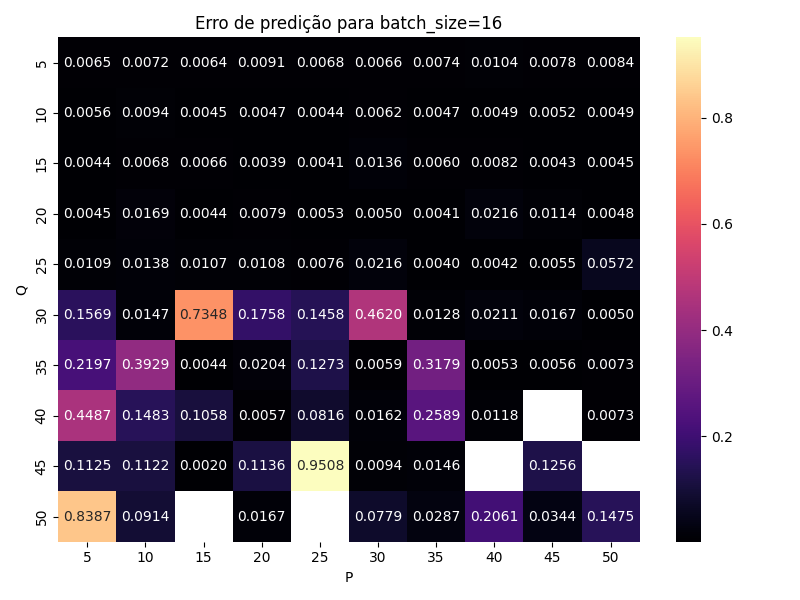
\includegraphics[width=0.7\linewidth]{Imagens/chap04/experiment_hp_metrics_16.png}
    \hfill
    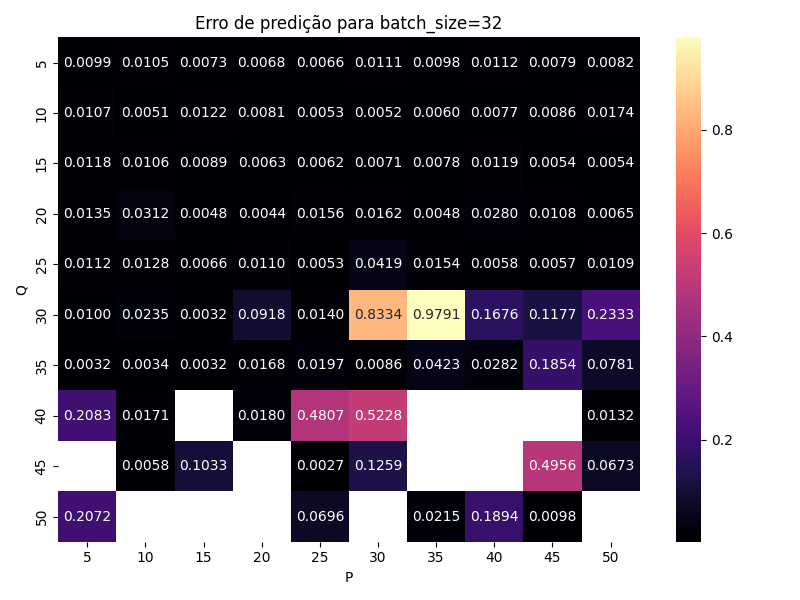
\includegraphics[width=0.7\linewidth]{Imagens/chap04/experiment_hp_metrics_32.png}
    \hfill
    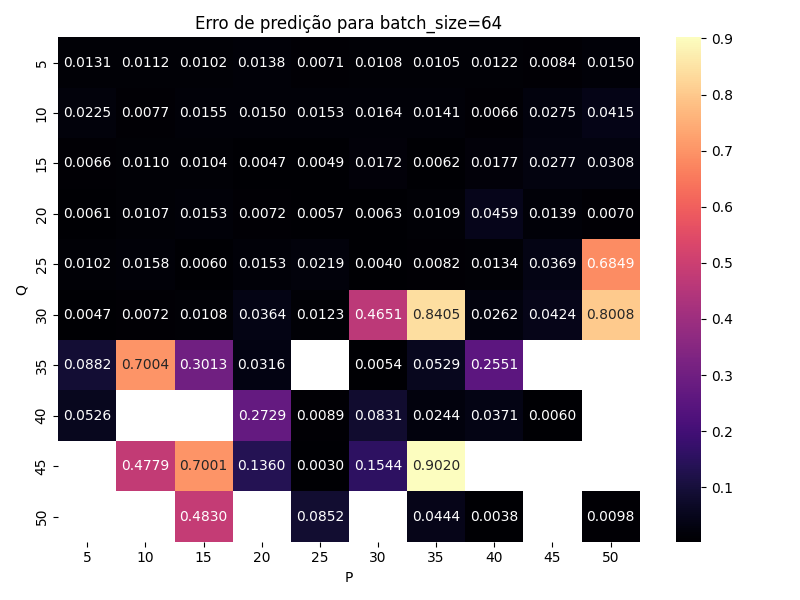
\includegraphics[width=0.7\linewidth]{Imagens/chap04/experiment_hp_metrics_64.png}
    \caption{Mapa de calor indicando o erro RMS para diferentes valores de $P$ e $Q$ e para tamanho de batelada 16 (esquerda), 32 (direita) e 64 (baixo). Fonte: Autor}
    \label{fig:exp_hp_metrics}
\end{figure}

O melhor resultado é o de $(P,Q,batch\_size)=(15,45,16)$, cujo RMSE é de 0.002. A predição dos modelos escolhidos estão descritas abaixo.

\subsection{Predição}
\subsubsection{Simulação}
A figura \ref{fig:lstm_prediction} mostra a predição das saídas do processo utilizando esta rede, num horizonte de 1000 pontos.
\begin{figure}[hbt!]
    \centering
    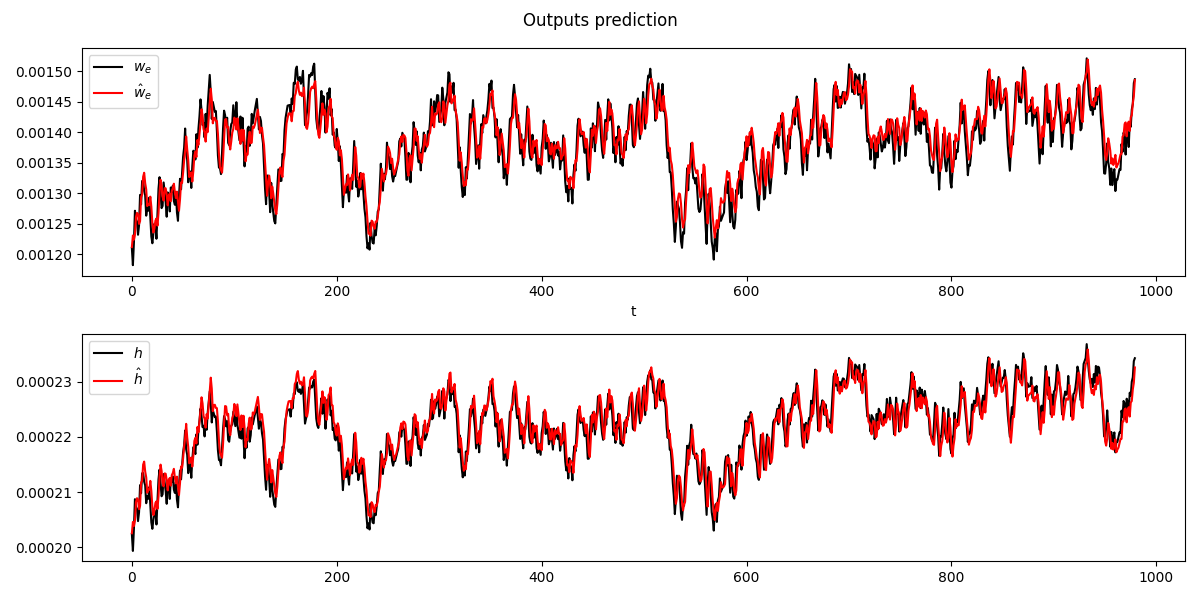
\includegraphics[width=0.7\linewidth]{Imagens/chap04/simulation_lstm_prediction.png}
    \caption{Predição das duas saídas do processo GMAW utilizando a rede com hiperparâmetros $P=20$, $Q=25$ e tamanho de batelada 16. Fonte: Autor}
    \label{fig:sim_lstm_prediction}
\end{figure}

A performance da rede é extremamente satisfatória, mostrando que foi capaz de modelar o processo e que se torna necessário interessante modificar a modelagem do distúrbio. Na figura \ref{fig:sim_error_histogram} está contido o histograma do erro de predição de cada saída, com a respectiva média, desvio padrão e p-valor do teste de normalidade. 

\begin{figure}[hbt!]
    \centering
    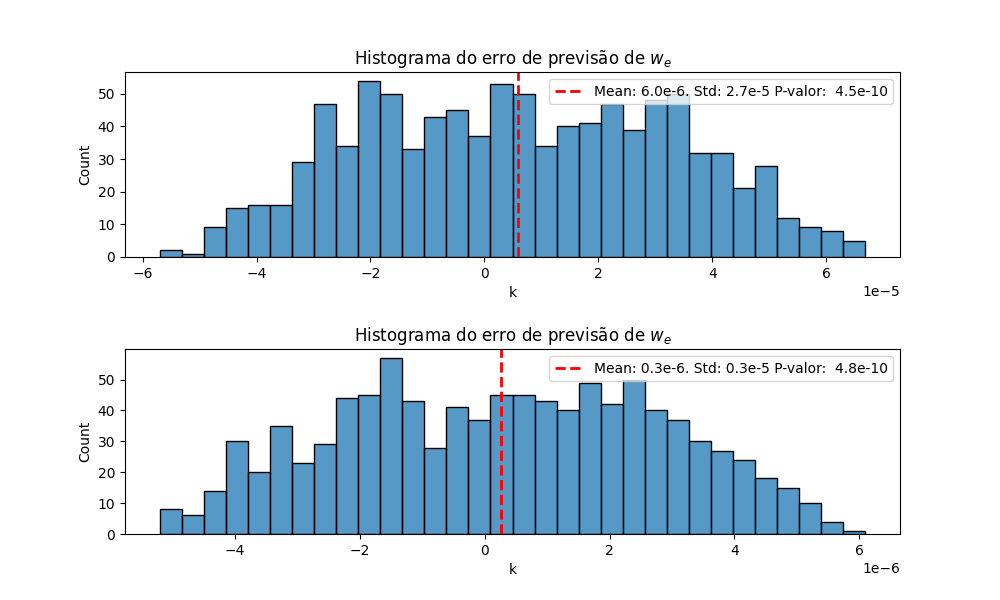
\includegraphics[width=0.7\linewidth]{Imagens/chap04/simulation_error_histogram.png}
    \caption{Histograma do erro de predição de cada saída, indicando a média, desvio padrão e valor-p do teste de normalidade Shapiro \cite{shapiro1965analysis}. Fonte: Autor.}
    \label{fig:sim_error_histogram}
\end{figure}

Nota-se que, para ambas as saídas, o ruído de predição é normal e de média próxima a zero, indicando que o modelo foi bem sucedido em modelar o processo dinâmico em questão.

\subsubsection{Dados experimentais}
A figura \ref{fig:lstm_prediction} mostra a predição das saídas do processo utilizando esta rede, num horizonte de 1000 pontos.
\begin{figure}[hbt!]
    \centering
    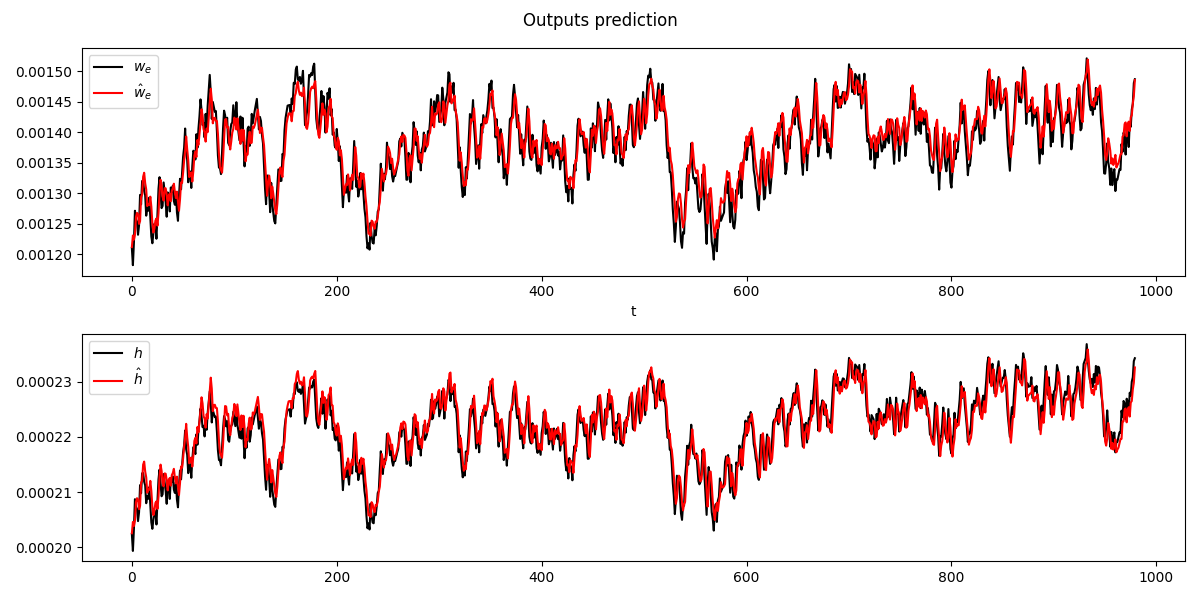
\includegraphics[width=0.7\linewidth]{Imagens/chap04/simulation_lstm_prediction.png}
    \caption{Predição das duas saídas do processo GMAW utilizando a rede com hiperparâmetros $P=20$, $Q=25$ e tamanho de batelada 16. Fonte: Autor}
    \label{fig:sim_lstm_prediction}
\end{figure}

A performance da rede é extremamente satisfatória, mostrando que foi capaz de modelar o processo e que se torna necessário interessante modificar a modelagem do distúrbio. Na figura \ref{fig:sim_error_histogram} está contido o histograma do erro de predição de cada saída, com a respectiva média, desvio padrão e p-valor do teste de normalidade. 

\begin{figure}[hbt!]
    \centering
    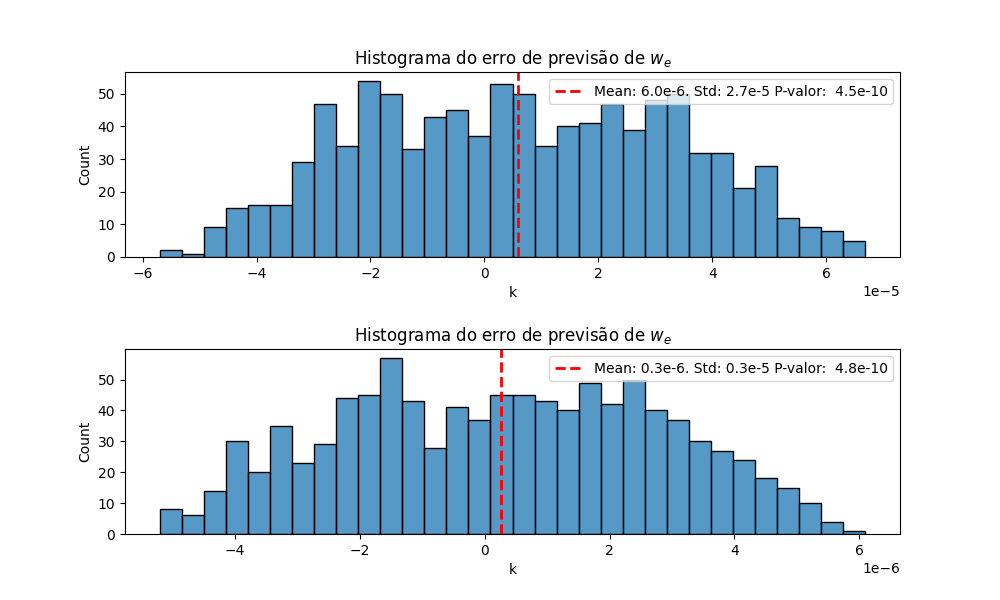
\includegraphics[width=0.7\linewidth]{Imagens/chap04/simulation_error_histogram.png}
    \caption{Histograma do erro de predição de cada saída, indicando a média, desvio padrão e valor-p do teste de normalidade Shapiro \cite{shapiro1965analysis}. Fonte: Autor.}
    \label{fig:sim_error_histogram}
\end{figure}

Nota-se que, para ambas as saídas, o ruído de predição é normal e de média próxima a zero, indicando que o modelo foi bem sucedido em modelar o processo dinâmico em questão.


\section{Controle MPC}
As figuras \ref{fig:mpc_inputs} e \ref{fig:mpc_outputs} ilustram os sinais de controle otimizados via MPC e as saídas controladas, respectivamente. 

\newpage
\begin{figure}[hbt!]
    \centering
    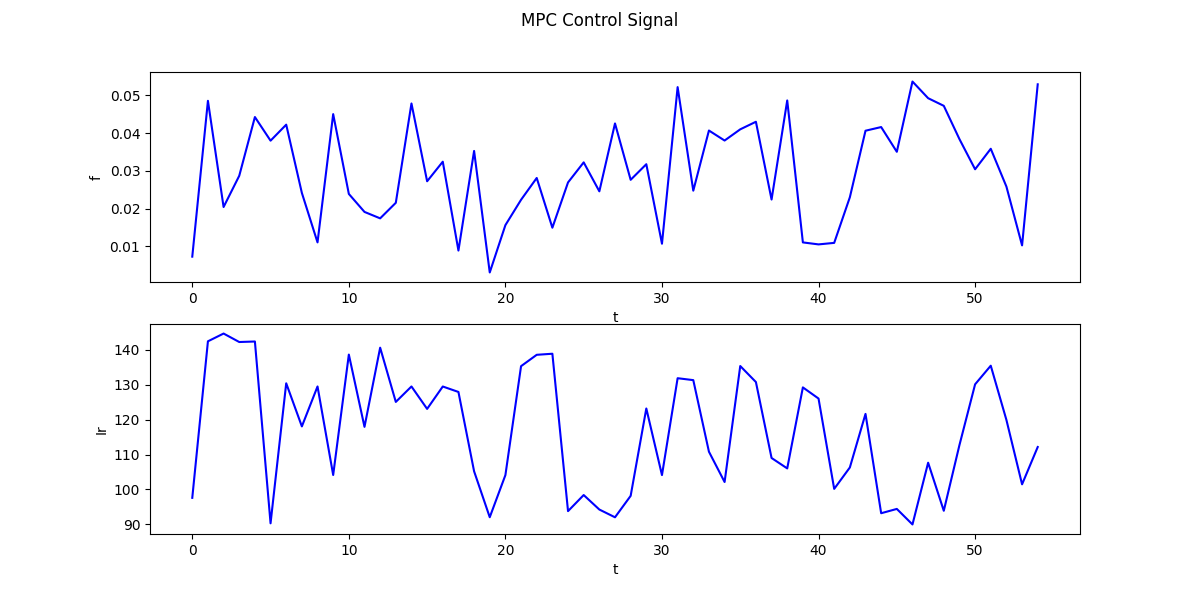
\includegraphics[width=0.7\linewidth]{Imagens/chap04/mpc_inputs.png}
    \caption{Sinais de controle via MPC. Fonte: Autor.}
    \label{fig:mpc_inputs}
\end{figure}

\begin{figure}[hbt!]
    \centering
    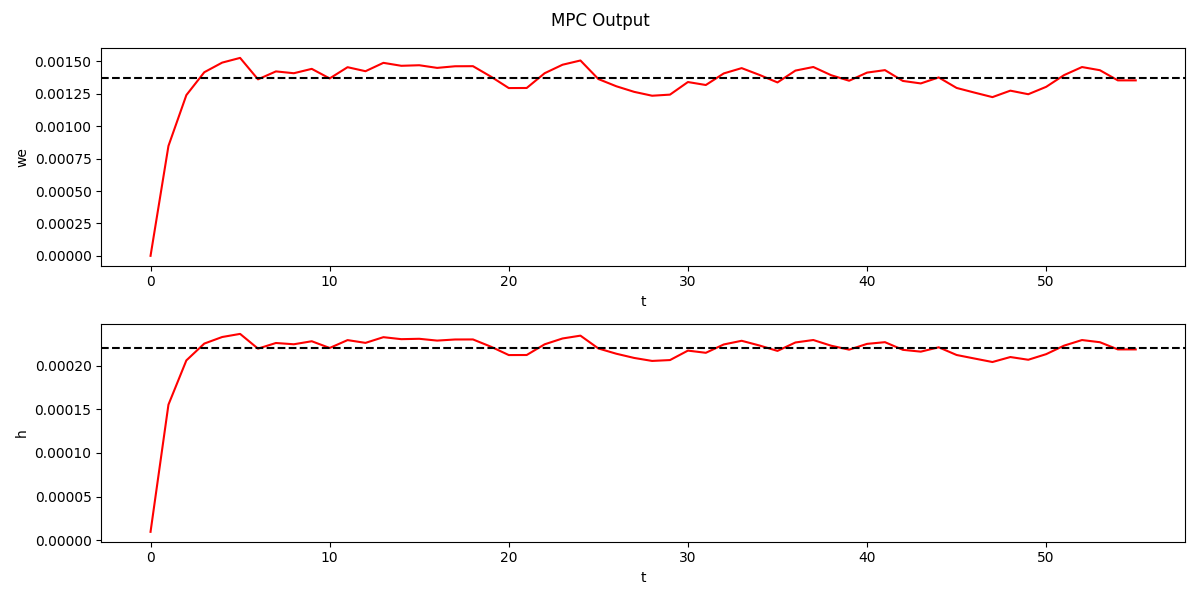
\includegraphics[width=0.7\linewidth]{Imagens/chap04/mpc_outputs.png}
    \caption{Saías controladas pelo MPC. Fonte: Autor.}
    \label{fig:mpc_outputs}
\end{figure}

A implementação foi capaz de controlar as saídas em torno de um referencial determinado. A oscilação de controle e saída estão dentro do aceitável considerando os limites físicos do processo. A tabela \ref{tab:metrics_mpc} descreve as métricas do controle do processo.

\newpage
\begin{table}[hbt!]
    \centering
    \begin{tabular}{c c c c}
         \hline
         Saída & Overshoot (\%) & RMSE & \Delta \bar{u} / u_{max} (\%) \\
         \hline
         $w_e$ & 12.82 & 6.28 \cdot 10^{-9} & 1.8\\
         $h$ & 8.14 & 7.23 \cdot 10^{-11} & 1.4 \\
         \hline
    \end{tabular}
    \caption{Métricas de controle MPC do processo GMAW estabalecido}
    \label{tab:metrics_mpc}
\end{table}